\documentclass[../main.tex]{subfiles}
\begin{document}

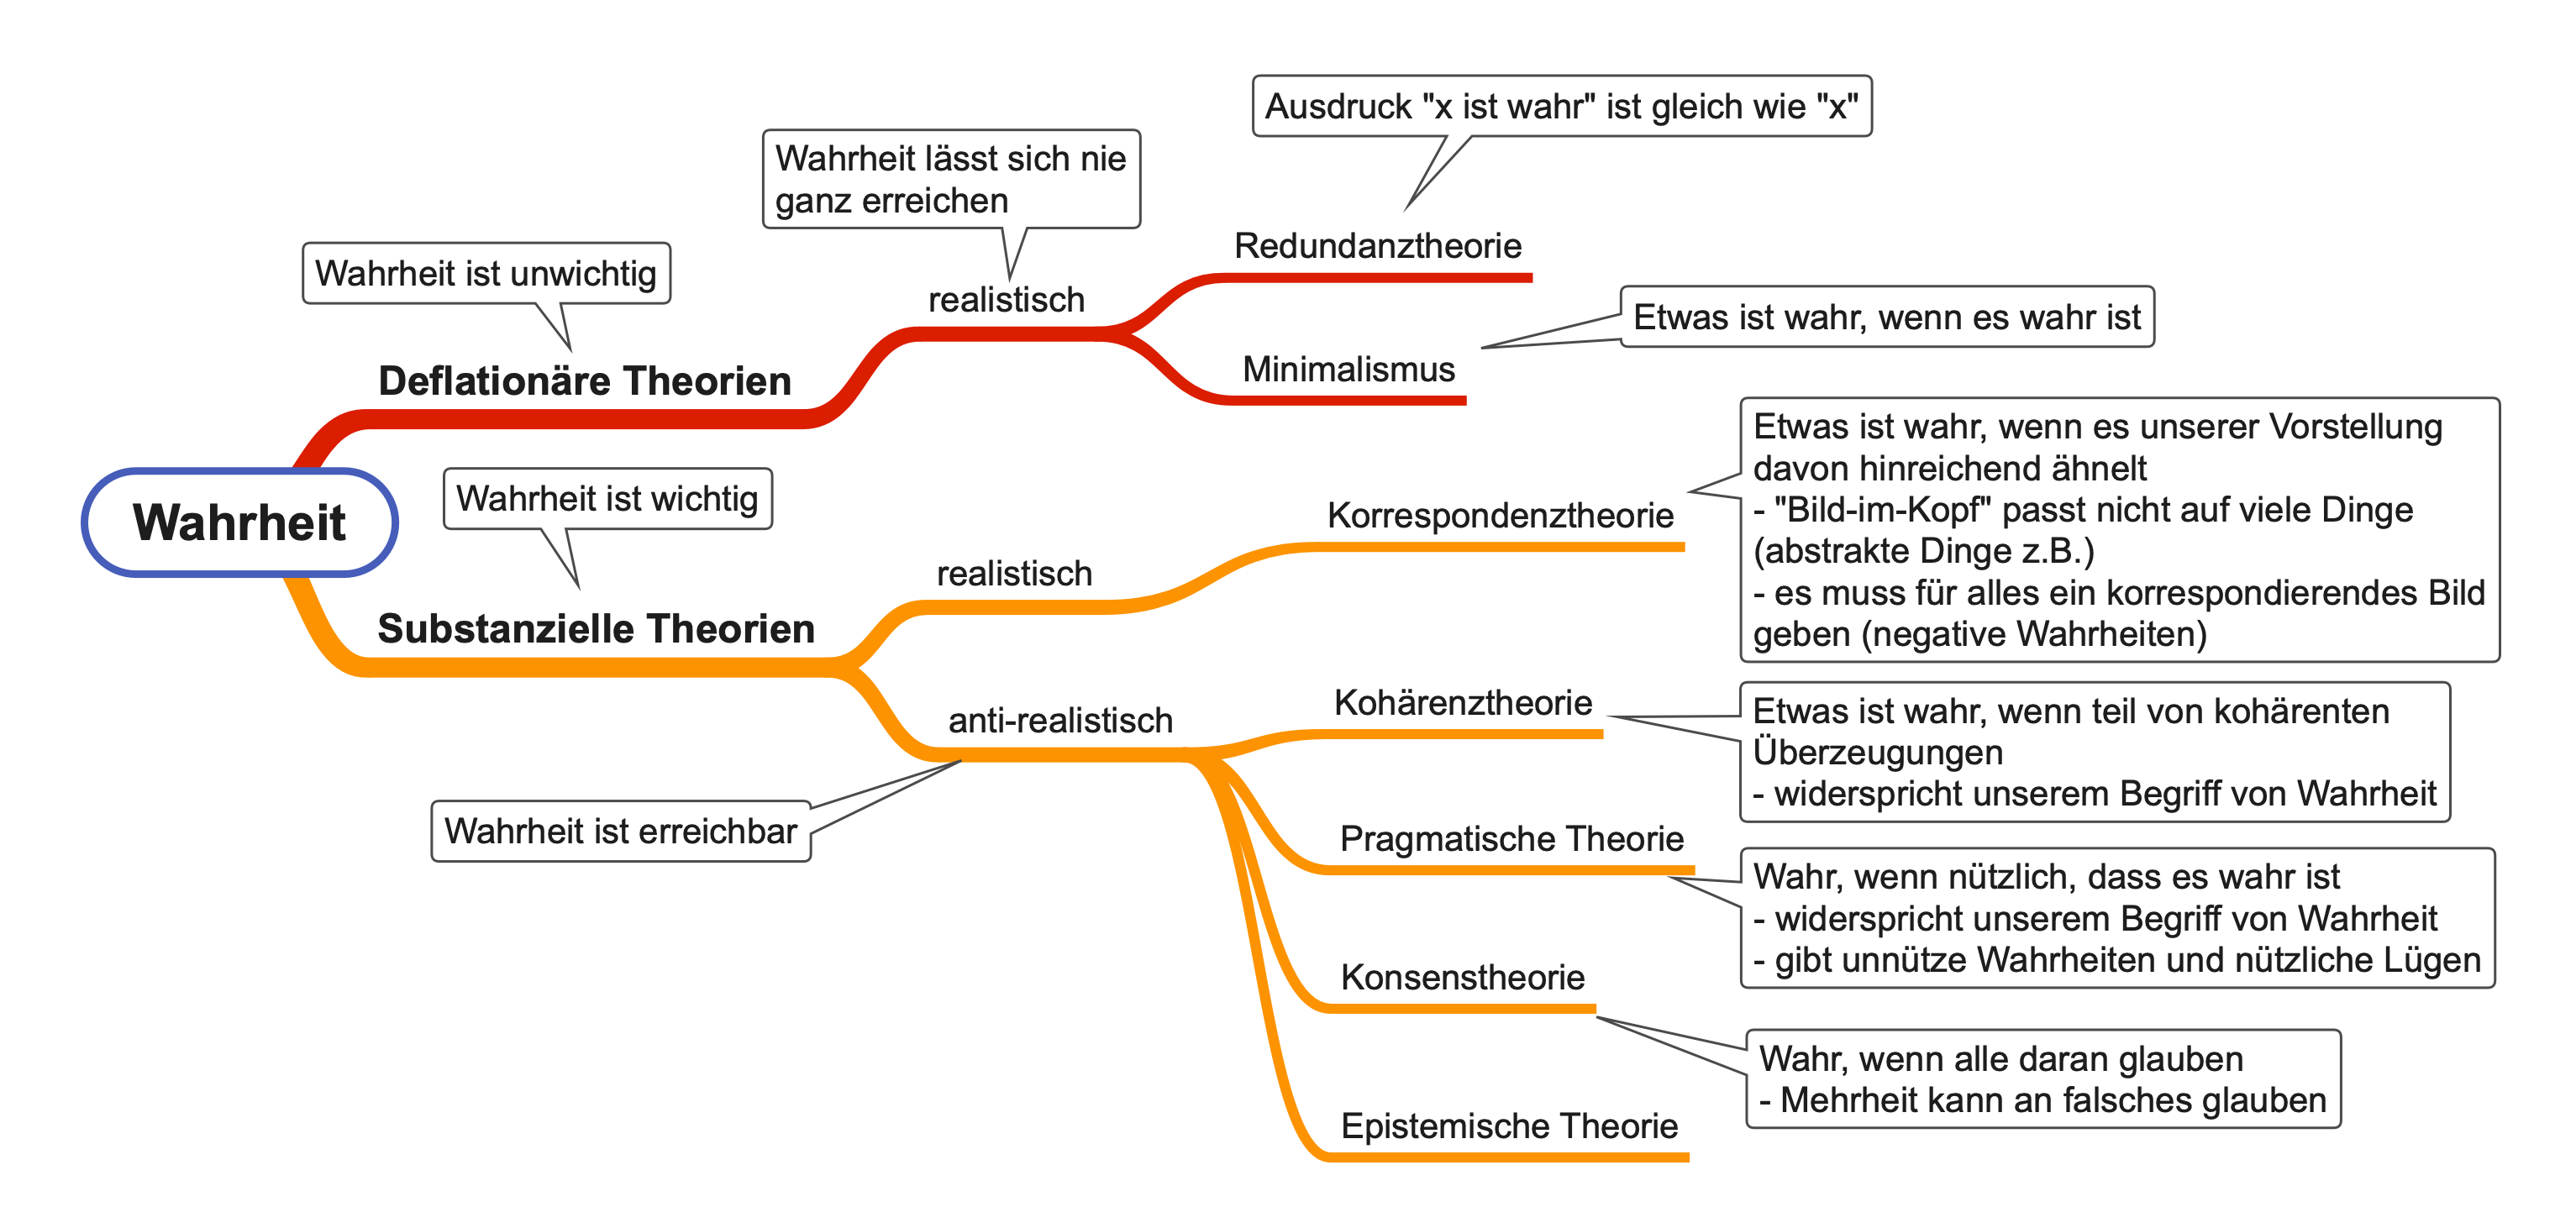
\includegraphics[width=\textwidth]{images/Wahrheit_Uebersicht.png}

\vspace{20pt}

Die Wahrheitstheorie beantwortet Fragen wie <<Was ist Wahrheit?>>, <<Was heisst es, wahr zu sein?>> oder <<Welche Bedungen muss etwas erfüllen, um als wahr gelten zu können?>>. Die Wahrheitstheorien liefern aber keine Wahrheit über spezifische Dinge oder geben uns konkrete Eigenschaften, an denen Wahrheit gemessen werden kann. Bei der Beantwortung der Fragen wird der Fokus auf den \textit{Wahrheitswertträger} (Was hat einen Wahrheitswert?) und dessen Legitimation gelegt. 

\textit{Wahrheitswertträger} können verschiedene Dinge sein. In der Psychologie können dies Überzeugungen oder Urteile sein, in der Linguistik sprachliche Objekte (Äusserungen) oder in dem Platonismus abstrakte Entitäten, d.h. Propositionen (Sinn\textsubscript{F}). Diese Aufteilung hat Einfluss auf wie wir über das Thema diskutieren können. Vertreter des Psychologismus oder des Lingualismus halten die inneren Überzeugungen als Träger, Aussagen/Propositionen sind lediglich Medium der Übertragung. Vertreter des Platonismus auf der anderen Seite halten die abstrakten Propositionen (etwas sagbares oder denkbares) für die \textit{Wahrheitswertträger}. In der Philosophie hat man sich darauf geeinigt, dass Propositionen (da zumindest nützlich) als Träger behandelt werden. 

\vspace{10pt}

\section{Typen von Wahrheitstheorien}
Abgsehen von der Frage nach dem Wahrheitsträger, unterscheidet man Wahrheitstheorien mit den folgenden Fragen:
\begin{itemize}
	\item Ist die Wahrheit (das Wahr-Sein) eine substantielle Eigenschaft der Wahrheitswertträger?
	\item Ist die Wahrheit abhängig vom menschlichen Denken und Erkennen?
\end{itemize}

\vspace{10pt}
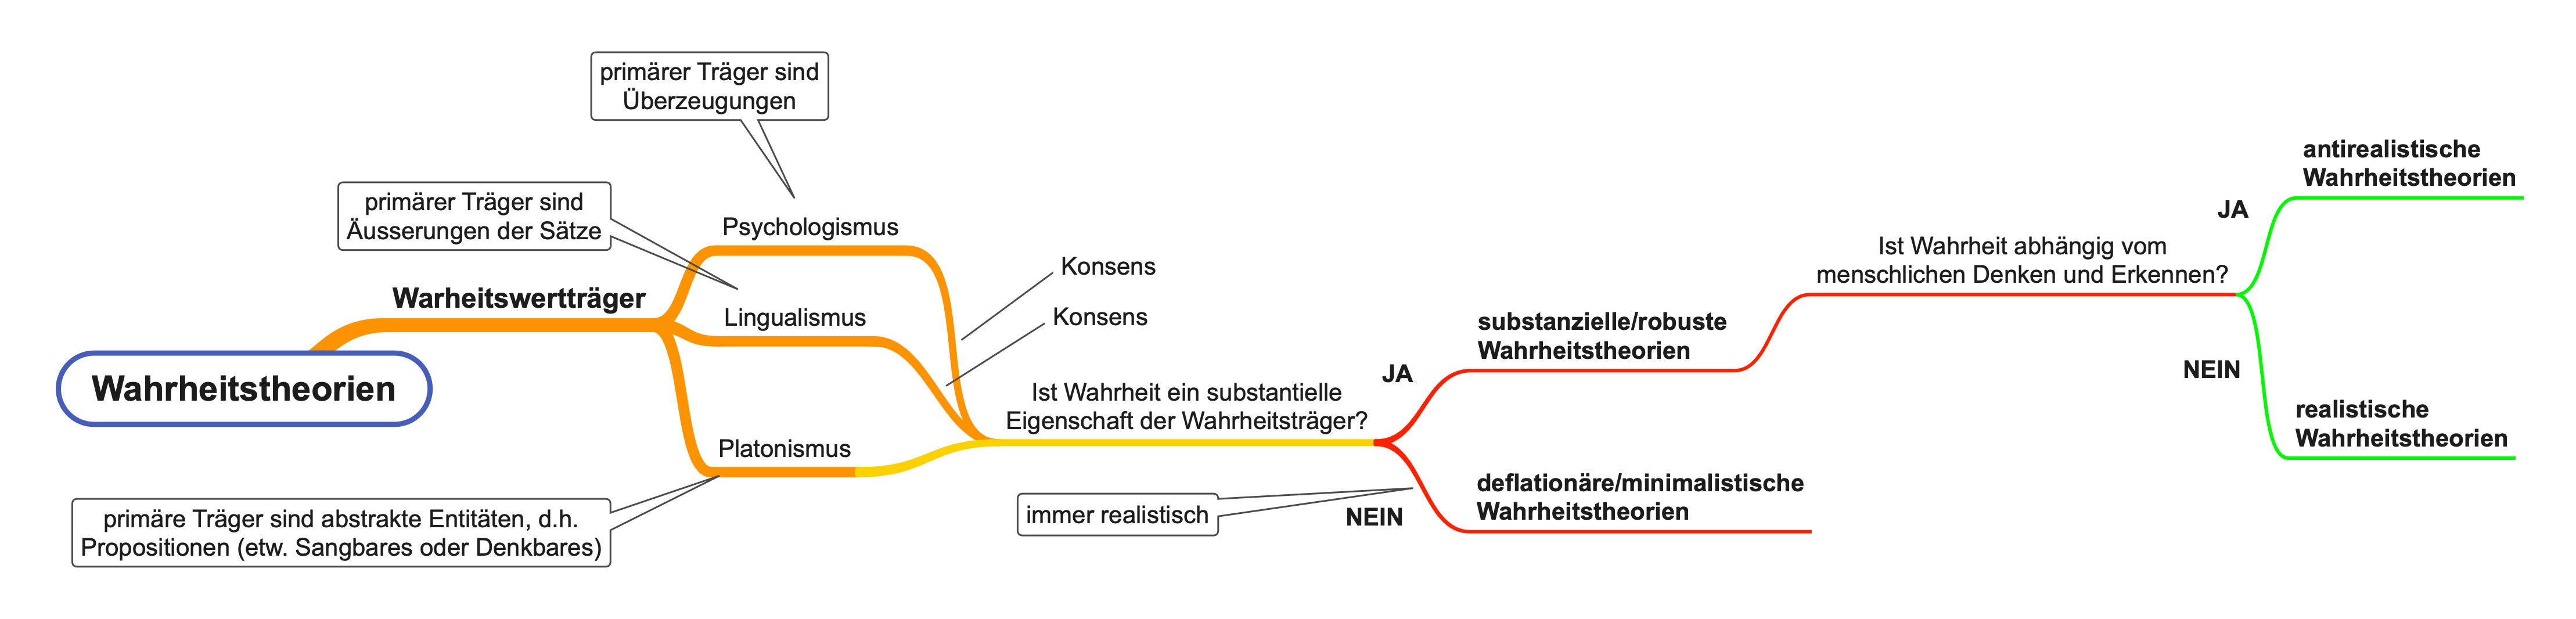
\includegraphics[width=\textwidth]{images/Wahrheitstheorien_Ueberblick.png}

\paragraph{Substanzielle Wahrheitstheorien} interpretieren die Wahrheit als zentraler Baustein verschiedenster Fachgebiete und schreiben ihr eine sehr hohe Gewichtung zu. Vertreter sind: 
\begin{enumerate}[label=(\alph*)]
	\item die unter den \textit{realistischen} Theorien angesiedelte \textbf{Korrespondenztheorie} (Thomas von Aquin, Bertrand Russel, evtl. Aristoteles), die besagt, dass eine Proposition p wahr ist, gdw. sie mit dem Verstand von Dingen übereinstimmt (\textit{adaequatio intellectus et rei}). Wahrheit steht also in einer Korrespondenzrelation (Mathematik: Eine Funktion weist mehrere Funktionswerte einer Zielmenge zu) zur Aussage.
	\item die unter den \textit{anti-realistischen} Theorien angesiedelte \textbf{Kohärenztheorie} (vgl. Hegel, Britische Idealisten), die besagt, dass eine Proposition p wahr ist, gdw. sie ein Teil eines kohärenten Überzeugungssystems ist. Eine Überzeugung ist kohärent, gdw. sie (1) widerspruchsfrei und (2) in einem engen Netz rationaler Beziehungen angesiedelt ist.
	\item die unter den \textit{anti-realistischen} Theorien angesiedelte \textbf{Pragmatistische Theorie} (vgl. William James), die besagt, dass Propositionen p wahr sind, gdw. es nützlich ist, zu glauben, dass sie wahr sind.
	\item die unter den \textit{anti-realistischen} Theorien angesiedelte \textbf{Konsenstheorie}, die besagt, dass Propositionen wahr sind, gdw. eine grosse Mehrheit aller Menschen glaubt, dass sie wahr sind. 
	\item die unter den \textit{anti-realistischen} Theorien angesiedelte \textbf{Epistemische Theorie} (Charles Sander Peirce), die besagt, dass eine Proposition p wahr ist, gdw., angenommen wir untersuchen die Proposition beliebig lang und mit den besten Methoden, wir zum Schluss kommen, dass sie wahr ist.    
\end{enumerate}
\paragraph{Deflationäre Wahrheitstheorien} versuchen zu zeigen, dass der Wahrheitsbegriff entweder nicht relevant ist oder er zumindest kein (philosophisches) Problem darstellt. In anderen Worten: \textit{Wahr-Sein} ist keine substanzielle Eigenschaft von Wahrheitsträgern (Es ist wahr, dass p, genau dann wenn p). Gemäss diesen Theorien ist es wahr, dass der Mond die Erde umkreist genau dann, wenn der Mond die Erde umkreist. Somit sind die deflationären Wahrheitstheorien \textit{realistische Positionen}. Vertreter sind:
\begin{enumerate}[label=(\alph*)]
	\item die als \textit{moderate deflationistisch} eingestufte \textbf{Redundanztheorie}, die besagt, dass ein Satz <<X ist wahr>> gleichbedeutend mit <<X>> ist. Demzufolge ist der Begriff <<wahr>> redundant und wir können ihn verlustlos aufgeben. 
	\item der als \textit{radikal deflationistisch} eingestufte \textbf{Minimalismus}, der besagt, dass die Feststellung <<Es ist wahr, dass p, gdw. p>> eine erschöpfende Feststellung ist. D.h. es benötig nicht mehr, resp. es ist alles, was über Wahrheit zu sagen gibt. Jedoch spielt <<wahr>> als Ausdruck eine wichtige Rolle in quantifizierten Sätzen wie <<Alles, was ich sage, ist wahr>> oder in opaken Wahrheitszuschreibungen wie <<Das, was er sagt, ist wahr>>. 
\end{enumerate}

\section{Alethischer Realismus}
\paragraph{These} Wahrheit geht über menschliche Erkenntnis hinaus. Ob eine Proposition wahr ist, hängt davon ab, wie die Dinge sind, also \textit{wie es sich verhält} (Wittgenstein, Tractatus 4.062). 

\paragraph{Erklärung} Der Alethische Realismus ist eine realistische Position, deren bekanntester Vertreter die Korrespondenztheorie ist. Der Irrtum, dass die Korrespondenztheorie der einzige Vertreter des alethischen Realismus ist, motiviert jedoch anti-realistische Positionen. Diese verstricken sich dabei aber oft in begrifflichen Wahrheiten. Das bedeutet, dass 

\section{Realistische Korrespondenztheorie}
\paragraph{These} Die Überzeugung, dass p, steht in einer Korrespondenzrelation zur Tatsache, dass p. Das bedeutet, dass eine Proposition wahr ist, wenn sie der Welt hinreichend ähnlich ist. 
\paragraph{Erklärung} Unter Korrespondenz versteht man die \textit{Relation der Ähnlichkeit} wie sie zum Beispiel zwischen einem Foto und der fotografierten Person besteht. Für Aussagen heisst dass, dass eine Aussage p (<<die Katze sitzt auf der Matte) wahr ist, weil es der Tatsache p (<<eine Katze sitzt auf einer Matte>>) hinreichend ähnlich ist. Somit unterstellt die Korrespondenztheorie jeder Aussage/Überzeugung/Proposition, dass es eine zugehörige Tatsache gibt, die mit ihr in einer korrespondierenden Beziehung steht. 
\paragraph{Probleme}
\begin{enumerate}
	\item Es ist zweifelhaft, ob zwischen einer Überzeugung (<<Bild im Kopf>>) und der Tatsache in der Welt überhaupt relevante Ähnlichkeiten bestehen. Kann man alle Gedanken als <<Bild im Kopf>> vor Augen führen und mit der Welt vergleichen?
	\item Ähnlichkeitsbeziehungen scheinen im Falle von visuellen Eindrücken noch eher plausibel zu sein. Doch wie sieht es aus, wenn abstrakte, negative oder konditionale Wahrheiten mit der Welt verglichen werden? Diese können kaum als <<Bilder im Kopf>> dargestellt werden. Und es scheint noch schwieriger zu sein, diese mit der Realität zu vergleichen. Beispiele dafür sind <<$2+2=4$>> oder <<Es gibt keine Einhörner>> oder <<Wäre der Mond aus Käse, wäre er essbar>>. 
	\item Wenn die Wahrheit einer Aussage durch die Beziehung zwischen der Aussage und der Welt besteht, so muss es für jede Aussage eine korrespondierende Tatsache geben. Für abstrakte, negative oder konditionale Wahrheiten müssten also auch Tatsachen existieren (die Tatsache, dass keine Einhörner existieren). Dies scheint unplausibel. 
\end{enumerate}

\subsection{Zweite Version der Korrespondenztheorie}
\paragraph{These} Betrand Russel und Ludwidg Wittgenstein: Korrespondenz ist eine \textit{strukturelle} Ähnlichkeits- oder Abbildungsbeziehung zwischen (1) Elementen der Sprache und des Denkens und (2) Elementen der Realität (Eigenschaften, Einzeldingen), aus denen Tatsachen zusammengesetzt sind.
\paragraph{Probleme}
\begin{enumerate}
	\item Auch der zweite Vorschlag gibt keine Anleitung, wie abstrakte, negative oder konditionale Wahrheiten in der Welt aussehen.
	\item Und es scheint nach wie vor unplausibel, dass es abstrakte, negative oder konditionale Tatsachen in der Wirklichkeit gibt. 
\end{enumerate}

\subsection{Dritte Version der Korrespondenztheorie}
\paragraph{These} Die Korrespondenzrelation ist primitiv (dies wird nicht weiter erklärt).
\paragraph{Probleme} 
\begin{enumerate}
	\item Es wird nicht erklärt, worin die Korrespondenzrelation besteht. Dies ist unbefriedigend. 
	\item Und es scheint nach wie vor unplausibel, dass es abstrakte, negative oder konditionale Tatsachen in der Wirklichkeit gibt. 
\end{enumerate}

\section{Anti-realistische Konsenstheorie}
\paragraph{These} Eine Proposition ist wahr, gdw. die Mehrheit aller Menschen glaubt, dass sie wahr ist.
\paragraph{Erklärung} Die Konsenstheorie der Wahrheit ist nicht lediglich ein Zusammenfinden und dann Abstimmen, was man als wahr betrachtet oder nicht. Sie soll eher als Diskurstheorie interpretiert werden; Menschen kommen zusammen und bringen Beweise und Argumente, die andere von einem Sachverhalt überzeugen und als Endergebnis stimmen die Leute mit denen Meinungen überein, die am besten bewiesen und für die am besten argumentiert wurde.
\paragraph{Probleme} 
\begin{enumerate}
	\item Es ist möglich, dass (1) eine grosse Mehrheit der Menschen daran glaubt, dass etwas wahr ist, obwohl es nicht wahr ist. Gleichzeitig (2) ist es möglich, dass etwas wahr ist, obwohl die grosse Mehrheit der Menschen nicht glaub, dass etwas wahr ist. Unser Begriff von Wahrheit widerspricht dem jedoch; Wie kann es sein, dass etwas wahr ist, obwohl es falsch sein könnte, nur weil die Mehrheit der Menschen glaubt, dass es wahr ist?
\end{enumerate}

\section{Anti-realistische Kohärenztheorie}
\paragraph{These} Eine Proposition ist wahr, gdw. sie ein Teil eines kohärenten Überzeugungssystems ist. Eine Überzeugung ist kohärent, gdw. sie (1) widerspruchsfrei und (2) in einem engen Netz rationaler Beziehungen angesiedelt ist.
\paragraph{Probleme}
\begin{enumerate}
	\item Ebenso wie die Konsenstheorie und die Pragmatische Theorie widerspricht die Theorie unserem Begriff von Wahrheit; Wie kann es sein, dass etwas wahr ist, obwohl es falsch sein könnte, nur weil die Mehrheit der Menschen glaubt, dass es wahr ist?
\end{enumerate}

\section{Anti-realistische pragmatische Theorie}
\paragraph{These} Eine Proposition p ist wahr, gdw. es nützlich ist, zu glauben, dass sie wahr sind.
\paragraph{Probleme}
\begin{enumerate}
	\item Ebenso wie die Konsenstheorie und die Kohärenztheorie widerspricht die Theorie unserem Begriff von Wahrheit; Wie kann es sein, dass etwas wahr ist, obwohl es falsch sein könnte, nur weil es nützlich ist?
	\item Es gibt Dinge, die sind nicht nützlich, aber wahr. Umgekehrt gibt es Dinge, die sind falsch, aber nützlich. 
\end{enumerate}

\end{document}